\section{Date: 2026-07-22}
\noindent \textbf{Series ID: NNBICPA027N} 

\noindent This series is titled Nonfinancial Noncorporate Business; Withdrawals from Income of Quasi-Corporations, Paid, Transactions and has a frequency of Annual, End of Period. The units are Millions of U.S. Dollars and the seasonal adjustment is Seasonally Adjusted Annual Rate.The observation start date is 1959-01-01 and the observation end date is 2024-01-01.The popularity of this series is 1. \\ 

\noindent \textbf{Series ID: M1YTOTL1ST000} 

\noindent This series is titled Current-Cost Depreciation of Private and government fixed assets: Nonresidential: Structures and has a frequency of Annual. The units are Millions of Dollars and the seasonal adjustment is Not Seasonally Adjusted.The observation start date is 1925-01-01 and the observation end date is 2024-01-01.The popularity of this series is 1. \\ 

\subsection{Raw Regression}
\noindent Regresses the two series against each other directly. A significant result here can come just as easily from both series sharing a long-run trend as from any real relationship.

\begin{center}
\begin{tabular}{lclc}
\toprule
\textbf{Dep. Variable:}           & value\_fred\_M1YTOTL1ST000 & \textbf{  R-squared:         } &     0.985   \\
\textbf{Model:}                   &            OLS             & \textbf{  Adj. R-squared:    } &     0.984   \\
\textbf{Method:}                  &       Least Squares        & \textbf{  F-statistic:       } &     4111.   \\
\textbf{Date:}                    &      Wed, 22 Jul 2026      & \textbf{  Prob (F-statistic):} &  8.67e-60   \\
\textbf{Time:}                    &          13:16:17          & \textbf{  Log-Likelihood:    } &   -777.64   \\
\textbf{No. Observations:}        &               66           & \textbf{  AIC:               } &     1559.   \\
\textbf{Df Residuals:}            &               64           & \textbf{  BIC:               } &     1564.   \\
\textbf{Df Model:}                &                1           & \textbf{                     } &             \\
\textbf{Covariance Type:}         &         nonrobust          & \textbf{                     } &             \\
\bottomrule
\end{tabular}
\begin{tabular}{lcccccc}
                                  & \textbf{coef} & \textbf{std err} & \textbf{t} & \textbf{P$> |$t$|$} & \textbf{[0.025} & \textbf{0.975]}  \\
\midrule
\textbf{const}                    &   -1720.1069  &     5808.925     &    -0.296  &         0.768        &    -1.33e+04    &     9884.554     \\
\textbf{value\_fred\_NNBICPA027N} &       0.4156  &        0.006     &    64.115  &         0.000        &        0.403    &        0.429     \\
\bottomrule
\end{tabular}
\begin{tabular}{lclc}
\textbf{Omnibus:}       &  7.252 & \textbf{  Durbin-Watson:     } &    0.477  \\
\textbf{Prob(Omnibus):} &  0.027 & \textbf{  Jarque-Bera (JB):  } &   10.958  \\
\textbf{Skew:}          &  0.289 & \textbf{  Prob(JB):          } &  0.00417  \\
\textbf{Kurtosis:}      &  4.911 & \textbf{  Cond. No.          } & 1.31e+06  \\
\bottomrule
\end{tabular}
%\caption{OLS Regression Results}
\end{center}

Notes: \newline
 [1] Standard Errors assume that the covariance matrix of the errors is correctly specified. \newline
 [2] The condition number is large, 1.31e+06. This might indicate that there are \newline
 strong multicollinearity or other numerical problems.

\begin{figure}
\centering
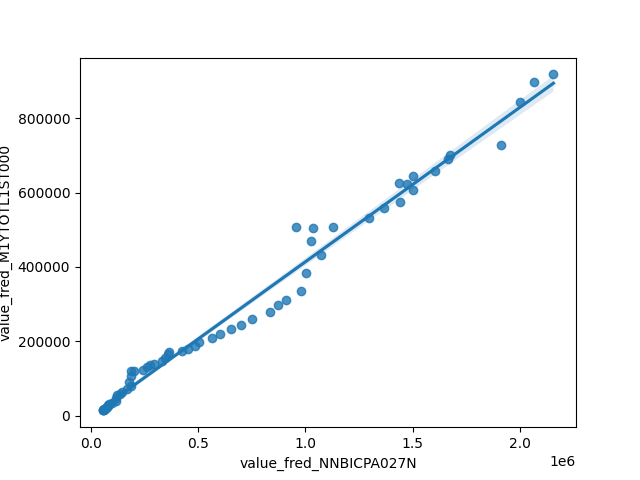
\includegraphics[scale = 0.9]{plots/plot_2026-07-22.png}
\caption{Raw Regression Plot for 2026-07-22}
\end{figure}
\newpage
\subsection{Detrended Regression}
\noindent Regresses the residuals of each series after removing its own linear time trend, so a shared trend can no longer drive the result on its own. A relationship that stays significant here is better evidence of a genuine link between the two series.

\begin{center}
\begin{tabular}{lclc}
\toprule
\textbf{Dep. Variable:}                      & value\_fred\_M1YTOTL1ST000\_detrended & \textbf{  R-squared:         } &     0.873   \\
\textbf{Model:}                              &                  OLS                  & \textbf{  Adj. R-squared:    } &     0.871   \\
\textbf{Method:}                             &             Least Squares             & \textbf{  F-statistic:       } &     439.3   \\
\textbf{Date:}                               &            Wed, 22 Jul 2026           & \textbf{  Prob (F-statistic):} &  2.31e-30   \\
\textbf{Time:}                               &                13:16:17               & \textbf{  Log-Likelihood:    } &   -777.37   \\
\textbf{No. Observations:}                   &                     66                & \textbf{  AIC:               } &     1559.   \\
\textbf{Df Residuals:}                       &                     64                & \textbf{  BIC:               } &     1563.   \\
\textbf{Df Model:}                           &                      1                & \textbf{                     } &             \\
\textbf{Covariance Type:}                    &               nonrobust               & \textbf{                     } &             \\
\bottomrule
\end{tabular}
\begin{tabular}{lcccccc}
                                             & \textbf{coef} & \textbf{std err} & \textbf{t} & \textbf{P$> |$t$|$} & \textbf{[0.025} & \textbf{0.975]}  \\
\midrule
\textbf{const}                               &    2.698e-09  &     3943.730     &  6.84e-13  &         1.000        &    -7878.507    &     7878.507     \\
\textbf{value\_fred\_NNBICPA027N\_detrended} &       0.4024  &        0.019     &    20.960  &         0.000        &        0.364    &        0.441     \\
\bottomrule
\end{tabular}
\begin{tabular}{lclc}
\textbf{Omnibus:}       &  5.762 & \textbf{  Durbin-Watson:     } &    0.463  \\
\textbf{Prob(Omnibus):} &  0.056 & \textbf{  Jarque-Bera (JB):  } &    8.362  \\
\textbf{Skew:}          &  0.128 & \textbf{  Prob(JB):          } &   0.0153  \\
\textbf{Kurtosis:}      &  4.725 & \textbf{  Cond. No.          } & 2.05e+05  \\
\bottomrule
\end{tabular}
%\caption{OLS Regression Results}
\end{center}

Notes: \newline
 [1] Standard Errors assume that the covariance matrix of the errors is correctly specified. \newline
 [2] The condition number is large, 2.05e+05. This might indicate that there are \newline
 strong multicollinearity or other numerical problems.

\begin{figure}
\centering
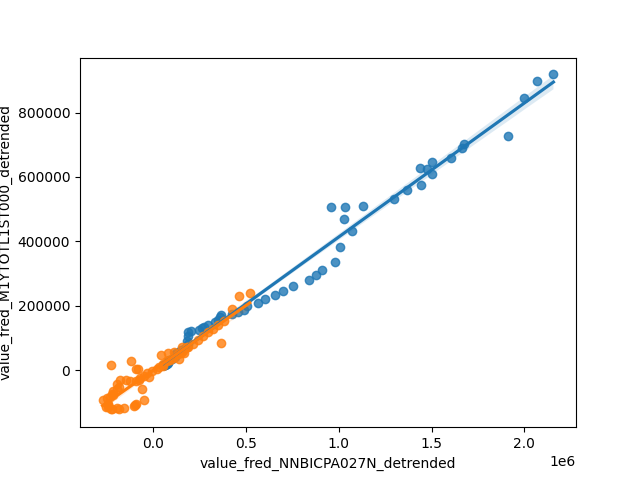
\includegraphics[scale = 0.9]{plots/plot_2026-07-22_detrended.png}
\caption{Detrended Regression Plot for 2026-07-22}
\end{figure}
\newpage
